\documentclass[12pt]{article}

% This first part of the file is called the PREAMBLE. It includes
% customizations and command definitions. The preamble is everything
% between \documentclass and \begin{document}.

\usepackage[margin=1in]{geometry}  % set the margins to 1in on all sides
\usepackage{graphicx}              % to include figures
\usepackage{amsmath,bm}            % great math stuff
\usepackage{amsfonts}              % for blackboard bold, etc
\usepackage{amsthm}                % better theorem environments
\usepackage{listings}
\usepackage{hyperref}
\usepackage{tikz}
\usepackage[]{algorithm2e}
\usepackage{parskip} 			   % no paragraph indentation

\usetikzlibrary{arrows,automata}


% various theorems, numbered by section

\newtheorem{thm}{Theorem}[section]
\newtheorem{lem}[thm]{Lemma}
\newtheorem{dfn}[thm]{Definition}
\newtheorem{prop}[thm]{Proposition}
\newtheorem{cor}[thm]{Corollary}
\newtheorem{conj}[thm]{Conjecture}

\DeclareMathOperator{\id}{id}

\newcommand{\bd}[1]{\mathbf{#1}}  % for bolding symbols
\newcommand{\RR}{\mathbb{R}}      % for Real numbers
\newcommand{\ZZ}{\mathbb{Z}}      % for Integers
\newcommand{\col}[1]{\left[\begin{matrix} #1 \end{matrix} \right]}
\newcommand{\comb}[2]{\binom{#1^2 + #2^2}{#1+#2}}

\lstset{ % General setup for the package
    language={[LaTeX]TeX},
    basicstyle=\footnotesize\sffamily,
    tabsize=4,
    columns=fixed,
    keepspaces,
    commentstyle=\color{red},
    keywordstyle=\color{blue},
    xleftmargin=.1\textwidth,
    xrightmargin=.1\textwidth
}

\begin{document}

\nocite{*}


\title{Randomized Algorithms \\
       Assignment 2}

\author{Viktor Hansen \& Simon Rueskov Schleicher}

\maketitle

\begin{abstract}
  This is the second weekly assignment for the Randomized Algorithms course offered at The Department of Computer Science, Uni. Copenhagen.
\end{abstract}

\pagebreak

\section*{Problems}

\subsection*{2.1}
We prove by induction over k that for any deterministic evaluation algorithm, there are instances of $T_{d,k}$ that forces the algorithm to read the values on all $d^{2k}$ leaves and the last leaf read determines whether the root is 1 or 0.\\
\\
Base step: for k=0 we only have one leaf, so any deterministic evaluation algorithm has to read them all. Furthermore that leaf is the root, so it determines whether the root is 1 or 0.\\
\\
Induction step: We assume it holds for any tree with size $k$, and need to show that it holds for any tree of size $k+1$. For a tree of size $k+1$, we have at the top a root that is an AND-note. Below that we have two OR-nodes, and below that we have 4 trees of size k. Since a deterministic evaluation algorithm looks at the nodes in a deterministic order, it also looks at the nodes in each of the subtrees in a specific order, and we can use the induction hypothesis.\\
There has to be one of the subtrees that are the first to get its last node inspected. We use the induction hypothesis and set the last node inspected in that subtree in the way that makes the root of that subtree 0. Since the parent to that root is an OR-node, we don't know yet whether it will be 1 or 0.\\
The 2nd subtree to get its last node inspected has 2 possibilities: Its root either shares a parent with the subtree we have already evaluated or it doesn't.\\
In the case where it shares a parent, we set the last node inspected in the way that makes the root 1. The parent OR-node can now look at a 1 and a 0, so the result is 1, but then we don't know the result of the AND-node in the root of the whole tree. We set the last node in the 3rd subtree to get fully evaluated in such a way that the root of that subtree is 0, and we have to inspect the 4th subtree. We can set the last node in the 4th subtree both so the root of the whole tree is 0 and so the root of the whole tree is 1.
In the case, where the 2nd subtree fully evaluated does not share a parent with the first, we set the last node in that subtree, so the root of the tree is 0, and we can't evaluate the parent OR-node. The 3rd subtree fully evaluated now either shares a parent with the first or the second subtree fully evaluated. We set the last node in the 3rd subtree in such a way that the root is 1, and we then have to also fully evaluate the 4th subtree before we can evaluate the root of the whole tree. Depending what we set the last node inspected in the 4th subtree, the root of the whole tree can both result in 0 or 1.\\
And we're done.

\subsection*{3.1}
Let $X$ be the number of empty bins after $m$ balls and $X_i$ be 1 if bin $i$ is empty after $m$ balls and 0 otherwise for $0\leq i\leq n$. For $X_i$ to be empty after m balls, we need all the m balls to land in a different bin, so we have $Pr[X_i]=\left(1-\frac{1}{n}\right)^m$ and $$E[X]=\Sigma_{i=0}^nE[X_i]=\Sigma_{i=0}^nPr[X_i]=\Sigma_{i=0}^n\left(1-\frac{1}{n}\right)^m=n\left(1-\frac{1}{n}\right)^m$$
For $m=n$ we get $$E[X]=n\left(1-\frac{1}{n}\right)^n\approx\frac{n}{e}$$

\subsection*{3.3(a)}
Let $X$ be the number of memory modules that has received exactly 1 memory request after $n$ memory requests has been sent and $X_i$ be 1 if memory module $i$ has received exactly 1 memory request after $n$ memory requests has been sent and 0 otherwise for $0\leq i\leq n$. We have $Pr[X_i]={n\choose 1}\left(\frac{1}{n}\right)^1\left(1-\frac{1}{n}\right)^{n-1}=\left(1-\frac{1}{n}\right)^{n-1}$.\\
Let $Y$ be the number of memory modules that has received exactly 2 memory request after $n$ memory requests has been sent and $Y_i$ be 1 if memory module $i$ has received exactly 2 memory request after $n$ memory requests has been sent and 0 otherwise for $0\leq i\leq n$. We have $Pr[Y_i]={n\choose 2}\left(\frac{1}{n}\right)^2\left(1-\frac{1}{n}\right)^{n-2}={n\choose 2}\frac{1}{n^2}\left(1-\frac{1}{n}\right)^{n-2}$.
Let $Z$ be the number of processors whose requests are satisfied. We have \begin{align*}E[Z]&=E[X]+2E[Y]=\left(\Sigma_{i=0}^nE[X_i]\right)+2\Sigma_{i=0}^nE[Y_i]=\left(\Sigma_{i=0}^nPr[X_i]\right)+2\Sigma_{i=0}^nPr[Y_i]\\&=\left(\Sigma_{i=0}^n\left(1-\frac{1}{n}\right)^{n-1}\right)+2\Sigma_{i=0}^n{n\choose 2}\frac{1}{n^2}\left(1-\frac{1}{n}\right)^{n-2}\\&=n\left(1-\frac{1}{n}\right)^{n-1}+2n\frac{n(n-1)}{2}\frac{1}{n^2}\left(1-\frac{1}{n}\right)^{n-2}=\frac{n}{1-\frac{1}{n}}\left(1-\frac{1}{n}\right)^n+(n-1)\left(1-\frac{1}{n}\right)^{n-2}\\&=\frac{n-1}{\left(1-\frac{1}{n}\right)^2}\left(1-\frac{1}{n}\right)^n+\frac{n-1}{\left(1-\frac{1}{n}\right)^2}\left(1-\frac{1}{n}\right)^n\approx\frac{2e(n-1)}{\left(\frac{n-1}{n}\right)^2}=\frac{2en^2}{n-1}\end{align*}
This is around $2en$, which is of course impossible (we can satisfy more processor than are available), so we must have made a mistake somewhere.

\pagebreak

\section*{Summary - April 27th and May 2nd}
\subsection*{Game tree evaluation}
Consider an algorithm for evaluating perfect, boolean, binary game trees with $n$ $0/1$-leaves consisting of AND-nodes (min) on even levels and OR-nodes (max) on uneven levels. Then
\\
\begin{thm}
Let $k$ denote the number of and-or levels in the tree, so that the height of the tree is $2k$ and the number of leaves is $n=4^k$. Then any det. algorithm might need to inspect all leaves and thus runs in $\Omega(n)$ or $\Omega(4^k)$ time in the worst case.
\end{thm}
We will give a rand. algorithm running in expected time $O(3^k) \approx O(n^{0.793})$. Let $T_w$ denote the subtree rooted at $w$ and $N_w$ be the number of leaves in $T_w$ inspected by the random. algorithm. Then we wish to show $\mathbf{E}\left[ N_r \right] \leq 3^k$ where $r$ is the root of such a game tree and do so by induction on $k \geq 0$. When $k=0$, $\mathbf{E}\left[ N_r \right] = 3^0 = 1 \leq 3^k$. Now for $k > 0$ we have
\begin{figure}[!ht]
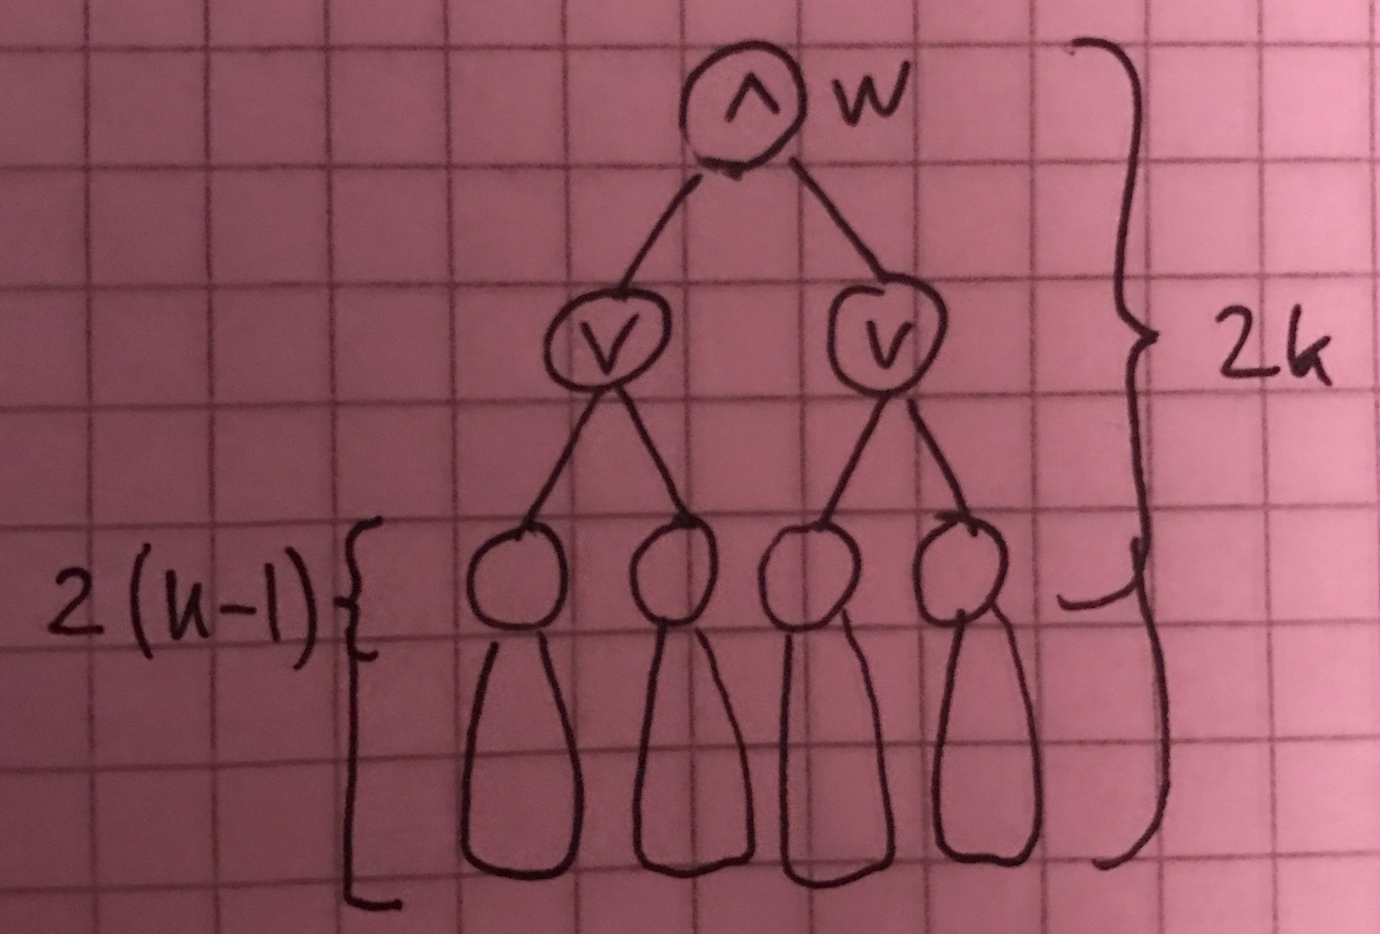
\includegraphics[width=8cm]{img/gametree.png}
\centering
\end{figure}

Consider child $u$ of $w$. Then in case $1$, both children are $0$ and the parent is an OR-node. Thus $\mathbf{E}\left[ N_u \right] \leq 2 \cdot 3^{k-1}$. In case $2$, one of the children are $1$ and another is $0$ and $\mathbf{E}\left[ N_u \right] \leq 3^{k-1} + \frac{1}{2} \cdot 3^{k-1} = \frac{3}{2} \cdot 3^{k-1}$. Next, consider the root node $w$. In case $1$, one child node is $0$ and the other is $1$ and $\mathbf{E}\left[ N_w \right] \leq \frac{1}{2} \cdot \left( 2 \cdot 3^{k-1} \right) + \frac{1}{2} \cdot \left( \frac{3}{2} \cdot 3^{k-1} + 2 \cdot 3^{k-1} \right) < 3^k$. In case $2$, both child nodes return $1$ and $\mathbf{E}\left[ N_w \right] \leq 2 \cdot \frac{3}{2} 3^{k-1} = 3^{k}$.

\subsection*{Game theory (von Neumann)}
Let $M$ be an $n \times n$ payoff-matrix in which each entry $M_{ij}$ denotes the payoff to the row player from the column player when the row player chooses strategy $i$ and the column player chooses strategy $j$.
\\
\begin{dfn}
(Pure strategies) Define the values for row and column-player as $V_R = \max\limits_{i} \min\limits_{j} M_{ij}$ and $V_C = \min\limits_{j} \max\limits_{i} M_{ij}$, respectively
\end{dfn}

In general $V_R \leq V_C$ and when $V_R=V_C$ the game has a solution.
\\
\begin{dfn}
(Mixed strategies) Strategy for row player is a prob. dist. over the rows of $M_{ij}$, $\overline{p}=\left( p_1, \hdots, p_n \right)$ and similarly for the column player with $\overline{q}$ over the columns in place of $\overline{p}$. Define the values for the row-player as $V_R = \max\limits_{\overline{p}} \min\limits_{\overline{q}} \sum \sum p_i \cdot q_j \cdot M_{ij}$ and $V_C = \min\limits_{\overline{q}} \max\limits_{\overline{p}} \sum \sum p_i \cdot q_j \cdot M_{ij}$
\end{dfn}
The following theorem shows that mixed-strategy games always have a solution \\
\begin{thm}
(von Neumann) For any game and any mixed strategies $\overline{p}$ and $\overline{q}$, $V_R = V_C$
\end{thm}
And the following theorem shows that the optimal mixed strategy, given the other player chooses a pure strategy always results in an equal payoff \\
\begin{thm}
(Loomis) $\max\limits_{\overline{p}} \min\limits_j \sum p_i M_{ij} = \min\limits_{\overline{q}} \max\limits_i \sum q_j M_{ij} $
\end{thm}

\subsection*{Yao's Minimax Principle}
Given a finite set $\mathcal{I}$ of problem instances all of the same size and a finite set, $\mathcal{A}$, of det. algorithms for $\mathcal{I}$, let $C(I,A)$ denote the cost associated with running $A \in \mathcal{A}$ on a problem instance $I \in \mathcal{I}$
\begin{figure}[!ht]
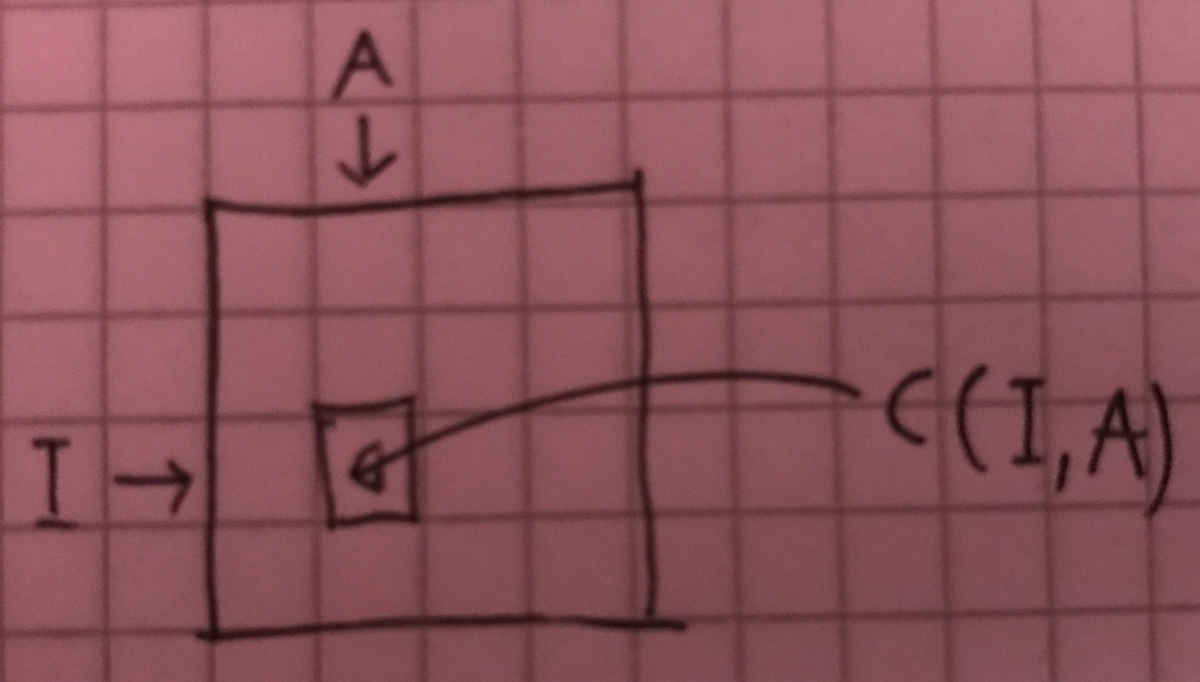
\includegraphics[width=8cm]{img/payoffmatrix}
\centering
\end{figure}
\begin{thm}
(Yao's Minimax Principle) Given dists. $\overline{p}$ and $\overline{q}$, let $I_{\overline{p}}$ be picked from $\mathcal{I}$ according to $\overline{p}$, dually for $A_{\overline{q}}$. Then $\min\limits_{A \in \mathcal{A}} \mathbf{E}\left[ C(I_{\overline{p}}, A) \right] \leq \max\limits_{I \in \mathcal{I}} \mathbf{E} \left[ C(I, A_{\overline{q}}) \right]$
\paragraph{Proof:} $\min\limits_{A \in \mathcal{A}} \mathbf{E}\left[ C(I_{\overline{p}}, A) \right] = \min\limits_{A \in \mathcal{A}}\limits \sum\limits_{I \in \mathcal{I}} \overline{p}(I) \cdot C(I_{\overline{p}}, A) \leq \sum\limits_{A \in \mathcal{A}} \overline{q}(A) \sum\limits_{I \in \mathcal{I}} \overline{p}(I) \cdot C(I_{\overline{p}}, A) = \sum\limits_{I \in \mathcal{I}} \overline{p}(I) \sum\limits_{A \in \mathcal{A}} \overline{q}(A) \cdot C(I_{\overline{p}}, A) \leq \max\limits_{I \in \mathcal{I}} \mathbf{E} \left[ C(I, A_{\overline{q}}) \right]$
\end{thm}

\subsection*{Lower bound for game tree evaluation}
Choose $\overline{p}$: Independently, set each leaf to $1$ with prob. $p=\frac{3-\sqrt{5}}{2}$. $p$ satisfies $p=(1-p)^2$. Change tree to NOR tree. This does not change the semantics of the tree. \\
\begin{lem}
After fixing leaves according to $\overline{p}$, each node of $T$ is $1$ with prob. $p$.
\paragraph{Proof:} $P[w\text{ set to } 1] = (1-p)^2 = p$.
\end{lem}

\subsection*{Derandomization}
Consider boolean func. $f : \left\{ 0,1 \right\}^* \rightarrow \left\{ 0,1 \right\}$. A rand. boolean circuit, $C$, computes $f$ if:
\begin{enumerate}
\item $\forall x_1, \hdots, x_n$ s.t. $f(x_1, \hdots, x_n) = 0$, $C$ outputs $0$.
\item $\forall x_1, \hdots, x_n$ s.t. $f(x_1, \hdots, x_n) = 1$, $C$ outputs $1$ for at least half of the $2^m$ assignments of values to $r_1, \hdots, r_m$.\\
\end{enumerate} 
\begin{dfn}
(Rand.) circuits $C_1, \hdots$ is a (rand.) circuit family for $f$ if $C_i$ computes $f$ for all $x_1, \hdots, x_i$. \\
\end{dfn}

\begin{dfn}
A circuit family $C_1, \hdots$ has polynomial size if $\forall n \left| C_n \right| \leq n^c$ where $c$ is a constant. \\
\end{dfn}

\begin{thm}
If $f$ has a polynomial sized random circuit family then $f$ has a polynomial sized deterministic circuit family.

\paragraph{Proof:} Given $n$, for each $C_n$, construct table $T$ with a row for each $2^n$ choices of $x_1, \hdots, x_n$ and a column for each $2^m$ choices of $r_1, \hdots, r_m$. Now if $x \not\in L$ then $\forall r, C_n(x,r) = 0$ and if $x \in L$ then $C_{n}(x,r) = 1$ for at least half the choices of $r$.
\begin{enumerate}
\item Remove all rows where $f$ only outputs 0.
\item For each remaining row, at least half of the entries are 1, meaning that there must exist a column where at least half of the entries are 1. Construct circuit $T_1$ by hardwiring $r_1, \hdots, r_m$ to values for that column.
\item Remove rows having a 1 in the chosen column.
\item Construct $T_2$, $T_3, \hdots, T_k$ by repeating steps 2 and 3.
\item Output the OR of the circuits $T_1, \hdots, T_k$
\end{enumerate}
\end{thm}
We wish to bound the number of circuits and note that in each iteration we remove at least half of the rows of $T$. Hence $k \leq \log(2^n) = n$ the number of circuits in the deterministic circuit family is polynomial.

\subsection*{Balls into bins}
Given $n$ balls and $n$ bins, and ball $i$ goes into bin $j$ with probability $1/n$. Then the expected number of balls in bin $j$ is 1. Let $\varepsilon^=_j(k)$ denote the event where bin $j$ receives exactly $k$ balls. Then
\begin{align*}
\mathbf{Pr}\left[ \varepsilon^=_j(k) \right] = \binom{n}{k}\frac{1}{n}^n \left( 1-\frac{1}{n} \right)^{n-k} \leq \binom{n}{k}\frac{1}{n}^n \leq \binom{ne}{k}^k \left( \frac{1}{n} \right)^n = \left(\frac{e}{k}\right)^k 
\end{align*}
Now, let $\varepsilon^\geq_j(k)$ denote the event where bin $j$ receives $k$ or more balls, then
\begin{align*}
\mathbf{Pr}\left[ \varepsilon^\geq_j(k) \right] = \sum_{i=k}^{n} \mathbf{Pr}\left[ \varepsilon^=_j(i) \right] \leq \sum_{i=k}^{n} \left(\frac{e}{i}\right)^i \leq \sum_{i=k}^{n} \left(\frac{e}{k}\right)^i \leq \left(\frac{e}{k}\right)^k \sum_{i=0}^{\infty} \left( \frac{e}{k} \right)^i = \left( \frac{e}{k} \right)^k \frac{1}{1-\frac{e}{k}}
\end{align*}
Choosing $k^*=\frac{3 \ln n}{\ln \ln n}$ and inserting it into the above yields
\begin{align*}
\mathbf{Pr}\left[ \varepsilon_j^\geq(k^*) \right] \leq \frac{1}{n^2}.
\end{align*}
The probability of any bin receiving more than $k^*$ balls is given by
\begin{align*}
\mathbf{Pr}\left[ \cup_{j=1}^{n} \varepsilon_j^\geq(k^*) \right] \leq \sum_{j=1}^n \mathbf{Pr}\left[ \varepsilon_j^\geq(k^*) \right] \leq n \frac{1}{n^2} = \frac{1}{n}
\end{align*}

\subsection*{Markov's Inequality}
Given a non-negative random variable $Y$ and $t > 0$, then
\begin{align*}
\mathbf{Pr}\left[ Y \geq t \mathbf{E}\left[ Y \right] \right] \leq \frac{1}{t} \;\; \mathrm{ and } \;\; \mathbf{Pr}\left[ Y \geq t \right] \leq \frac{\mathbf{E}\left[ Y \right]}{t}
\end{align*}
To show the rightmost form, we get
\begin{align*}
\mathbf{E}\left[ Y \right] = \sum_{i} i \cdot \mathbf{Pr}\left[ Y=i \right] \geq \sum_{i \geq t} i \cdot \mathbf{Pr}\left[ Y=i \right] \geq t \cdot \sum_{i \geq t} \mathbf{Pr}\left[ Y=i \right] \geq t \cdot \mathbf{Pr}\left[ Y \geq i \right] 
\end{align*}
The leftmost form follows by substituting $t$ by $t \cdot \mathbf{E}\left[ Y \right]$ into the rightmost form.

\subsection*{Chebyshev's Inequality}
Given rand. var. $X$, define the variance of $X$, denoted by $\sigma^2$, as $\sigma^2 = \mathbf{E}\left[ \left( X - \mu_X \right)^2 \right]$, where $\mu_X = \mathbf{E} \left[ X \right]$. Now, given a random variable $X$ and $t > 0$, then
\begin{align*}
\mathbf{Pr}\left[ \left| X-\mu_X \right| \geq t\sigma_X \right] &= \mathbf{Pr}\left[ \left( X-\mu_X \right)^2 \geq t^2\sigma_X^2 \right] \\
&= \mathbf{Pr}\left[ \left( X-\mu_X \right)^2 \geq t^2 \mathbf{E}\left[\left( X-\mu_X \right)^2\right] \right] \\
&= \mathbf{Pr}\left[ Y \geq t^2\mathbf{E}\left[Y\right] \right] \\
&\leq \frac{1}{t^2}
\end{align*}
The last step follows from applying Markov's inequality.

\subsection*{Lazy Selection}
Refer to the algorithm given in the book. Let $S(k)$ denote the $k$th smallest element in $S$ and $r_{S(a)}$ denote the rank of $a$ in $S$. Any known det. alg. requires $\geq 3n$ comparisons to identify $S_{k}$. We want to show that \textsc{LazySelect} finds $S(k)$ with $2n + O(n)$ comparisons with prob. $1-O(n^{-1/4})$. The algorithm can err. if $S(k) < a$. For this to happen, fewer than $\mathcal{l}$ samples are smaller than $S(k)$ for $i=1, \hdots, n^{3/4}$, $X_i=1$ if $i$th sample $\leq S(k)$, and $X_i = 0$ otherwise. Let $X=\sum^{n^{3/4}}_{i=1} X_i$. We will bound the error probability using Chebyshev's inequality. We get $\mu_X = \sum^{n^{3/4}}_{i=1} \mu_{X_i} = n^{3/4}\cdot \frac{k}{n}=kn^{-1/4}$ and $\sigma_X^2 = \sum^{n^{3/4}}_{i=1} \sigma^2_{X_i} = n^{3/4}\frac{k}{n}\left( 1-\frac{k}{n} \right) \leq \frac{1}{4}n^{3/4}$ implying $\sigma_X \leq \frac{1}{2}n^{3/8}$ and
\begin{align*}
\mathbf{Pr} \left[ X \leq l \right] &= \mathbf{Pr} \left[ X \leq \mu_X - \sqrt{n} \right] = \mathbf{Pr} \left[ \mu_X - X \geq \sqrt{n} \right] \leq \mathbf{Pr} \left[ \left| \mu_X - X \right| \geq \sqrt{n} \right] \\
&\leq \mathbf{Pr} \left[ \left| \mu_X - X \right| \geq 2n^{1/8}\sigma_X \right] \leq \frac{1}{4n^{1/4}} = O(n^{-1/4})
\end{align*}
and hence the success probability is $\geq 1-O(n^{-1/4})$.

\subsection*{Two-point Sampling}
\begin{lem}
Let $a,b \in \mathbb{Z}_n$ where $n$ is a prime be picked independently and uniformly at random. Let $y_i = (a_i + b) \mod n$ for $i = 0, \hdots, n-1$. Then for all distinct $i,j \in \mathbb{Z}_n$, $y_i$ and $y_j$ are pairwise ind. and uniformly distributed in $\mathbb{Z}_n$. \\
\end{lem}

\begin{dfn}
Variables $X_1, \hdots, X_n$ are pairwise ind. iff. for all distinct $i,j$ and all $x_y$, $\mathbf{Pr}\left[ X_i = x \; | \; X_j = y \right] = \mathbf{Pr}\left[ X_i = x \right]$. \\
\end{dfn}

\begin{lem}
If $X_1, ... X_n$ are pairwise independent and $X = \sum X_{i=1}^n X_i$ then $\sigma^2_X = \sum_{i=1}^n \sigma_{X_i}^2$
\end{lem}

Given an algorithm $A(x,r)$ for deciding $L$ where $x \in L$ and $r$ is a random number in $\mathbb{Z}_n = \left\{ 0, \hdots, n-1 \right\}$ where $n$ is a prime s.t.
\begin{align*}
&\text{1) If } x \not\in L \text{ then } A(x,r) = 0 \; \forall r \in \mathbb{Z}_n \\
&\text{2) If } x \in L \text{ then } A(x,r) = 1 \text{ for at least half of the choices of } r \in \mathbb{Z}_n
\end{align*}
Simple method: Pick $t$ numbers, $r_i, \hdots, r_t$ independently and uniformly at random from $\mathbb{Z}_n$. Output $\lor_{i=1}^t A(x,r_i)$. Given $x \in L$ the failure probability $\leq 1/2^t$. For $t=2$, the failure probability $\leq 1/4$.

Two-point method: Now let $a,b \in \mathbb{Z}_n$ be picked uniformly at random. Let $r_i = (a_i + b) \mod n$, $Y_i = A(x, r_i)$ for $i = 0, \hdots, n-1$ and $Y=\sum_{i=0}^{n-1}Y_i$. We wish to bound $\mathbf{Pr}\left[ Y=0 \right]$ using Chebyshev's inequality. Now $\mu_{Y} = \sum^{n-1}_{i=0}\mu_{Y_i} \geq n/2$ and $\sigma_Y^2 = \sum_{i=0}^{n-1} \sigma^2_{Y_{i}} \geq n/4 \Rightarrow \sigma_Y \geq \sqrt{n}/2$. Inserting into Chebyshev's Inequality yields
\begin{align*}
\mathbf{Pr}\left[ Y = 0 \right] \leq \mathbf{Pr}\left[ \left| Y - \mu_Y \right| \geq \sqrt{n} \sigma_Y \right] \leq \frac{1}{n}
\end{align*}
which is better than $1/4$ for $n \geq 4$.

\end{document}
